\documentclass[conference]{IEEEtran}

%\usepackage{cite}

\usepackage[cmex10]{amsmath}
\usepackage{amssymb}

\usepackage{algorithm}
\usepackage{algorithmic}
\usepackage{indentfirst}
\renewcommand{\algorithmicrequire}{ \textbf{Initialization:}}
\renewcommand{\algorithmicensure}{ \textbf{Recurrence:}}

% Graph package
\ifx\pdfoutput\undefined
\usepackage{graphicx}
\else
\usepackage[pdftex]{graphicx}
\fi
\usepackage{epstopdf}

\usepackage{multirow}



% *** SUBFIGURE PACKAGES ***
\usepackage[tight,footnotesize]{subfigure}
% subfigure.sty was written by Steven Douglas Cochran. This package makes it
% easy to put subfigures in your figures. e.g., "Figure 1a and 1b". For IEEE
% work, it is a good idea to load it with the tight package option to reduce
% the amount of white space around the subfigures.


%\usepackage[caption=false]{caption}
%\usepackage[font=footnotesize]{subfig}
% subfig.sty, also written by Steven Douglas Cochran, is the modern
% replacement for subfigure.sty. However, subfig.sty requires and
% automatically loads Axel Sommerfeldt's caption.sty which will override
% IEEEtran.cls handling of captions and this will result in nonIEEE style
% figure/table captions. To prevent this problem, be sure and preload
% caption.sty with its "caption=false" package option. This is will preserve
% IEEEtran.cls handing of captions. Version 1.3 (2005/06/28) and later 
% (recommended due to many improvements over 1.2) of subfig.sty supports
% the caption=false option directly:
\usepackage[caption=false,font=footnotesize]{subfig}








% correct bad hyphenation here
\hyphenation{op-tical net-works semi-conduc-tor}


\begin{document}

% can use linebreaks \\ within to get better formatting as desired
\title{Efficient FPGA Implementation of\\ Overclocking Friendly Online Arithmetic Operators}


% author names and affiliations
%\author{\IEEEauthorblockN{Kan Shi, David Boland, and George A. Constantinides}
%\IEEEauthorblockA{Department of Electrical and Electronic Engineering\\
%Imperial College London\\London, UK\\
%\{k.shi11, david.boland03,g.constantinides\}@imperial.ac.uk}
%}

\maketitle


\begin{abstract}
%\boldmath
The abstract goes here.
\end{abstract}


% For peer review papers, you can put extra information on the cover
% page as needed:
% \ifCLASSOPTIONpeerreview
% \begin{center} \bfseries EDICS Category: 3-BBND \end{center}
% \fi
%
% For peerreview papers, this IEEEtran command inserts a page break and
% creates the second title. It will be ignored for other modes.
\IEEEpeerreviewmaketitle



\section{Introduction}

\section{Background: Online Arithmetic}
\subsection{Key Features of Online Arithmetic}
In conventional arithmetic, results are generated either from the least significant digit, e.g. addition and multiplication, or from the most significant digit, e.g. division and square root. This inconsistency in computing directions can result in large latency when propagating data among different operations. Online arithmetic was proposed to solve this problem [xxx]. With online arithmetic, both the inputs and the outputs are processed in a MSD-first manner. This enables parallelism and duplication among various operations, and the overall computation latency can be significantly reduced.

Online arithmetic was originally designed for digit-serial operation, of which the data flow is illustrated in Fig~\ref{Fig:OnlineDataFlow}. It can be seen that in order to generate the first output digit, $\delta$ digits of inputs are required and $\delta$ is called ``online delay''. Notice that $\delta$ is normally a constant, which is independent of the precision in a given operation. For ease of discussion, in the following of this paper the input data are normalized to fixed point numbers in the range $(-1,1)$. Based on this premise, the online representation of $N$-digit operands and result at iteration $j$ are given by (\ref{Eq:Online_Operands}), where $j\in[-\delta,N-1]$ and $r$ denotes the radix \cite{Ercegovac_Book}.

\begin{figure}[htbp]
  \centering
  %\vspace{-2.5ex}
  \includegraphics[width=.48\textwidth]{./Figures/OnlineArithmetic_DataFlow.pdf}
  %\vspace{-3ex}
  \caption{Dataflow in digit-serial Online Arithmetic. $\delta$ denotes the online delay.}
  %\vspace{-.5ex}
  \label{Fig:OnlineDataFlow}
\end{figure}

\begin{eqnarray}\label{Eq:Online_Operands}
\footnotesize
  X_{[j]}=\sum_{i=1}^{j+\delta}x_ir^{-i},~Y_{[j]}=\sum_{i=1}^{j+\delta}y_ir^{-i},~Z_{[j]}=\sum_{i=1}^{j}z_ir^{-i}
\normalsize
\end{eqnarray}

MSD-first operation is possible with the employment of the redundant number system \cite{RedundantNumber}, in which each digit is represented with a redundant digit set $\{-a, \cdots,-1,0, 1, \cdots, a\}$, where $a\in[r/2,r-1]$. Due to the redundancy, the MSDs of the result can be calculated only based on partial information of the inputs and then the value of the number can be revised by the following digits.

\subsection{Binary Online Addition}
Adders serve as a critical building block for arithmetic operations. To perform digit-parallel online addition, a redundant adder can be directly utilized. The adder structure diagram is shown in Fig~\ref{Fig:Radix2SD_adder}. A major advantage of the redundant number system over the standard ripple-carry based arithmetic is that the propagation of carry is eliminated, resulting in a precision-independent computation time for addition. As seen in Figure~\ref{Fig:Radix2SD_adder}, the computation delay of this adder is only 2 full adder (FA) delays for any operand word-length, with the cost of one extra FA for each digit of operands. This makes the online adder suitable for building up more complex arithmetic operators such as multipliers to accelerate the sum of partial products \cite{RedundantMult_1987}.

\begin{figure}[htbp]
	\centering
	\includegraphics[width=.5\textwidth]{./Figures/SDAdder.pdf}
%\vspace{-8.5ex}
	\caption{An $N$-digit binary digit-parallel online adder with $(N+1)$-digit outputs.}
	\label{Fig:Radix2SD_adder}
\end{figure}

In Section~\ref{Sec:OA_FPGA}, we will present a novel method of mapping the digit parallel online adder efficiently on FPGAs using the built-in carry resources.

\subsection{Binary Online Multiplication}
Multiplication is another key arithmetic operator. Typically the online multiplication is performed in a recursive digit-serial manner, as illustrated in Algorithm~\ref{Algorithm:OnlineMult} \cite{Ercegovac_OnlineMult} where both inputs and outputs are $N$-digit number as given in~(\ref{Eq:Online_Operands}). For a given iteration $j$, the product digit $z_j$ is generated through a selection function $sel()$. For the radix $r$ and a chosen digit set, there exits an appropriate selection method and a value of $\delta$ which ensure convergence \cite{Ercegovac_OnlineMult}. As radix-2 is used most commonly in computer arithmetic, we keep $r=2$ throughout this paper with the corresponding redundant digit set $\{\overline{1},0,1\}$. In this case $sel()$ is given by (\ref{Eq:SelFunc_OM}) \cite{Oregon_OnlineNetwork}. Notice that the election is made only based on 1 integer bit and 1 fractional bit of $W_{[j]}$.

\begin{algorithm}[tbp]
  \caption{Online Multiplication}
  \begin{algorithmic}[1]
    \REQUIRE~$X_{[-\delta]}=Y_{[-\delta]}=P_{[-\delta]}=0$
    \ENSURE~$for~~ j=-\delta,~-\delta+1,~\cdots,~N-1 ~~do$
      \begin{eqnarray}\label{Eq:OnlineMult_General}
        \begin{matrix}
          H_{[j]}   & = & r^{-\delta}\left(x_{j+\delta+1}\cdot Y_{[j+1]}+y_{j+\delta+1}\cdot X_{[j]}\right)\\
          W_{[j]}   & = & P_{[j]} + H_{[j]}\\
          z_j       & = & sel(W_{[j]})\\
          P_{[j+1]} & = & r\left(W_{[j]}-z_j\right)
        \end{matrix}
      \end{eqnarray}
  \label{Algorithm:OnlineMult}
  \vspace{-2ex}
  \end{algorithmic}
\end{algorithm}

\begin{eqnarray}\label{Eq:SelFunc_OM}
%\small
  sel(W_{[j]})=\begin{cases}
    1 & \text{ if } W_{[j]} \geqslant \frac{1}{2} \\
    0 & \text{ if } -\frac{1}{2}\leqslant W_{[j]}<\frac{1}{2} \\
    \overline{1} & \text{ if } W_{[j]}<-\frac{1}{2}
  \end{cases}
%\normalsize
\end{eqnarray}

In Section~\ref{Sec:OM_FPGA}, we will describe a modified online multiplication algorithm and its FPGA implementation, which are designed specifically targeting on digit parallel operations.

%\subsection{FPGA Architecture}


\section{Digit Parallel Online Adder on FPGAs}\label{Sec:OA_FPGA}
\subsection{Related Works}
There has been previous works focusing on efficient FPGA implementation of the digit-parallel online adder. Generally the existing approaches can be classified into three types:%, as discussed below. A more detailed review of current works can be found in xxx.
\begin{enumerate}
	\item efficient mapping of the digit-parallel online adder onto sophisticated FPGAs resources [xxx];
	\item multiple operands addition by designing compressor trees based on bit counters [xxx];
	\item modifying existing FPGA architecture for more efficient online addition [xxx] and for specific applications [xxx].
\end{enumerate}

Type 2 and type 3 are beyond the scope of this paper, as we focus on the general purpose online adder that takes 2 inputs and generate 1 outputs, as shown in Figure xxx. Specifically in type 1, both works took advantage of the built-in carry resources in FPGAs. Conventionally the ASIC implementation of online adders is based on the 4:2 compressors, as shown within the gray background in Figure xxx. However, directly applying this approach in the FPGAs could be less efficient. This is because there is no carry propagation between the 2 full adders within a 4:2 compressor, and the net delay between them can be large. Instead, Kamp et al and Ortiz et al described very similar mapping techniques for online adders with 2 different data representations, respectively. The main idea is to map the logic block within the dotted circle in Fig.~\ref{Fig:PreviousWork}. In this case, the fast-carry logic in the FPGA can be employed, and the delay between the 2 FAs is largely reduced. 

\begin{figure}[htbp]
	\centering
	\includegraphics[width=.5\textwidth]{./Figures/SDAdder_42comp_Spartan.pdf}
	\caption{Map the online adder onto Spartan FPGAs using the fast-carry resources. The grey background highlights the 4:2 compressor. Dotted circle indicates the logic block (LB) which can be mapped to the FPGA carry resources.}
	\label{Fig:PreviousWork}
\end{figure}

However, we notice the major limitations of both approaches that they only target on FPGAs with 4-input LUTs and 2 LUTs within a logic slice, such as the Xilinx Spartan series and the Altera Cyclone series. This is naturally reasonable because one LB can be mapped to a single slice. Nevertheless, for FPGAs with 6-input LUTs (6-LUT) and 4 LUTs in a slice, such as the Xilinx Virtex series and all Xilinx 7 series FPGAs, directly applying the approaches in [xxx] will result in either resource waste or logic fault. For instance, if 2 LBs are mapped to a slice with 4 LUTs as seen in Fig.~\ref{Fig:PreWorkVirtex6}s, the outputs of the second LB will be faulty because the its carry input cannot be explicitly initialized. 

\begin{figure}[htbp]
	\centering
	\includegraphics[width=.45\textwidth]{./Figures/SDadder_FastCarry_PreviousWork.pdf}
	\caption{Direct utilization of previous approaches on a Virtex-6 FPGA will results in faulty outputs.}
	\label{Fig:PreWorkVirtex6}
\end{figure}

\subsection{Proposed Mapping Method} 
To tackle this problem, we first modify the structure of the online adder to enable an efficient FPGA mapping. The structure of a 3-digit online adder is given as an example in Fig.~\ref{Fig:ModifiedOA}. In this equivalent structure, the first FA in each 4:2 compressor is split into 2 parts, which only generate carry and sum respectively. In this case they can be mapped individually on 2 LUTs. The second FA, which generates the outputs, is unchanged and can be implemented using the fast-carry logic.


%propose an alternative mapping method that targets on the slice containing 4 LUTs such as the Xilinx Virtex series and all Xilinx 7 series FPGAs. 

\begin{figure}[tbp]
	\centering
	\includegraphics[width=.5\textwidth]{./Figures/SDadder_FPGA_New.pdf}
	\caption{Modified structure of online adder. Left: an example of 3-digit online adder. The shaded part refers to the 2 logic blocks (LBs) that can be mapped onto 1 slice. Right: one LB. the dotted box outlines the logic that can be mapped onto 1 LUT and the corresponding fast-carry logic.}
	\label{Fig:ModifiedOA}
\end{figure}

The detailed slice mapping of the 2 LBs is shown in Fig.~\ref{Fig:SliceNew}. The I/O signals are identical to the previous example in Fig.~\ref{Fig:ModifiedOA}. It can be seen that a 6-LUT can be configured with two different output ports O6 and O5. For LB1, the carry input can be initialized by setting the O6 of LUT2 equal to 0 constantly. In this case, the output of MUXCY2 is O5 of LUT2, and the carry from LB2 will not affect the results of LB1. Using this mapping method the resources within 1 slice can be fully utilized, potentially leads to significant area reduction.  

\begin{figure}[tbp]
	\centering
	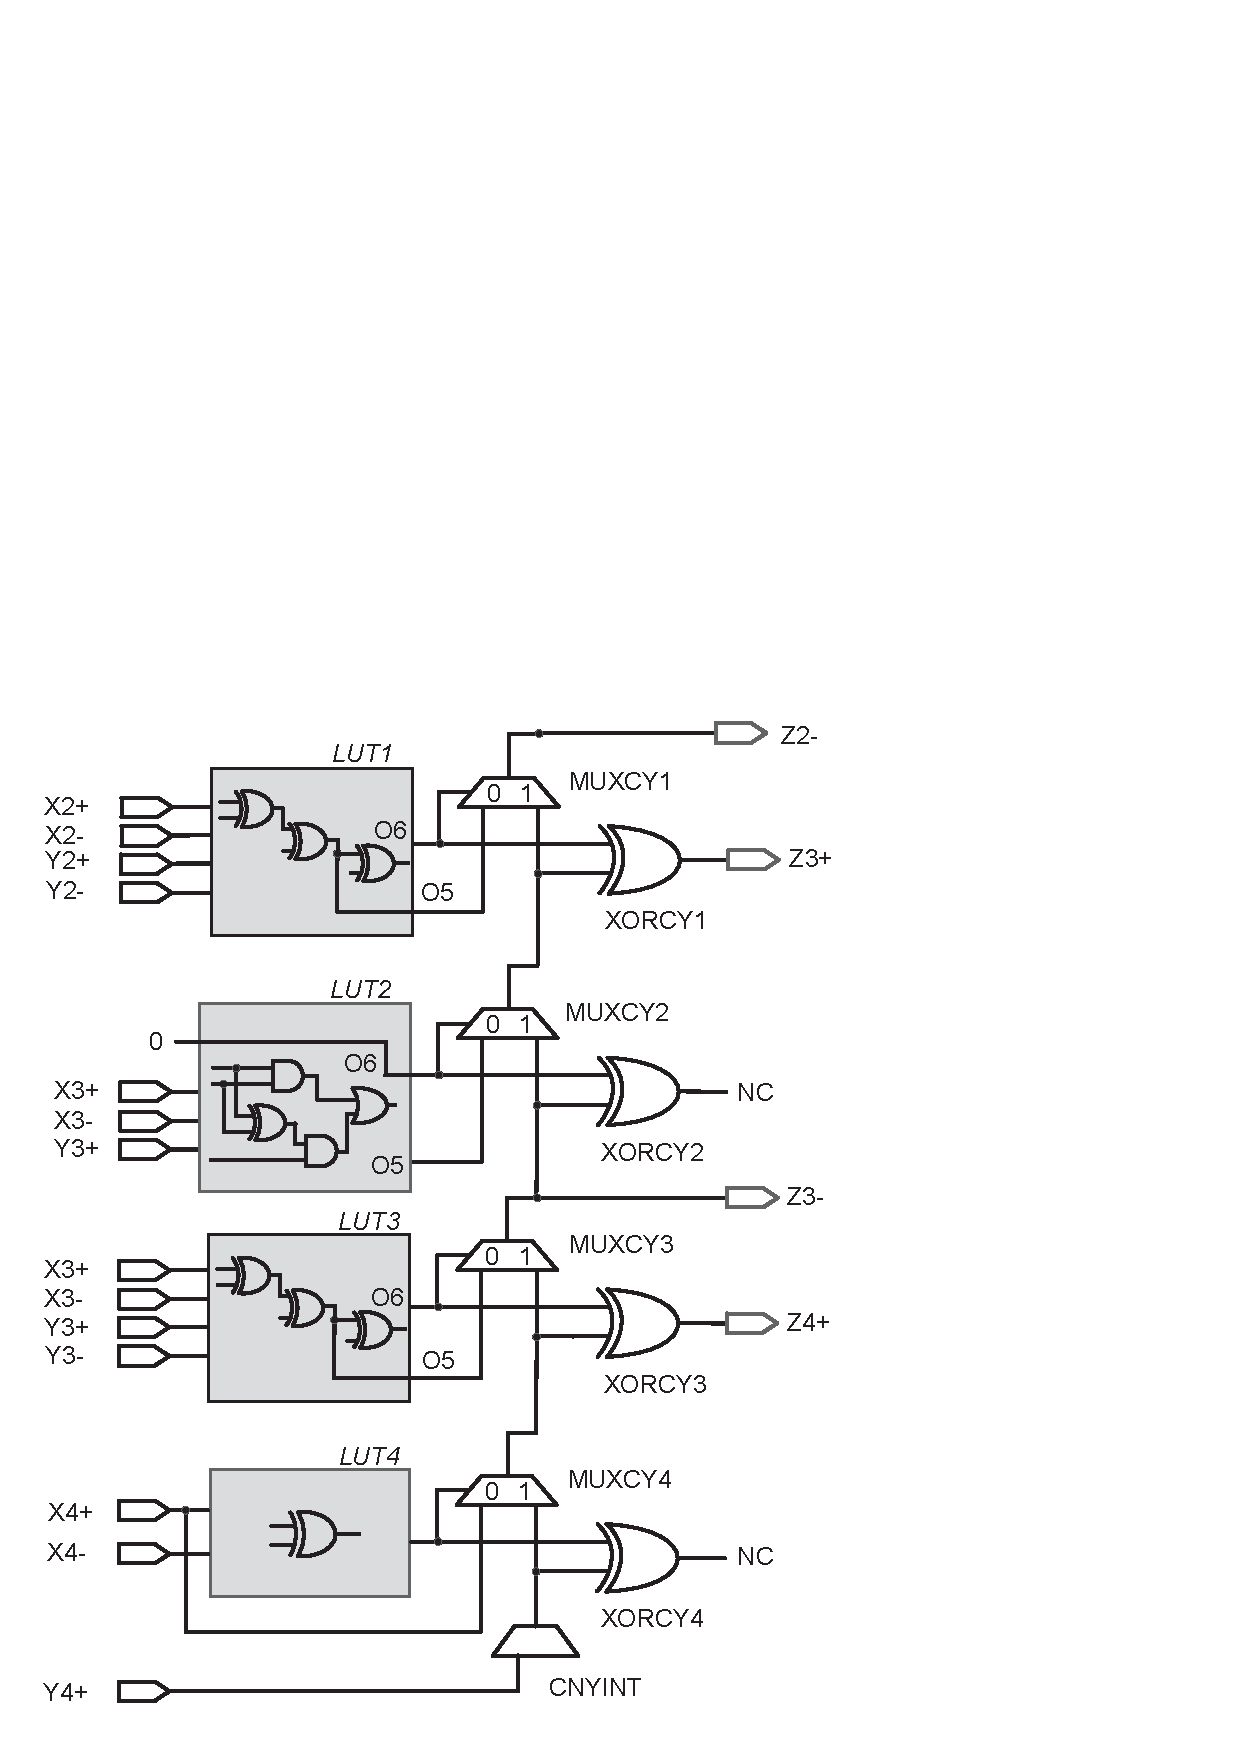
\includegraphics[width=.48\textwidth]{./Figures/SDadder_FastCarry_New.pdf}
	\caption{Implementation of 2 logic blocks (LBs) in 1 FPGA slice which contains four 6-LUTs. NC stands for ``Not Care''.}
	\label{Fig:SliceNew}
\end{figure}

\subsection{Performance Analysis}


\section{Digit Parallel Online Multiplier on FPGAs}\label{Sec:OM_FPGA}
\subsection{Algorithm of Digit Parallel Online Multiplication}
Algorithm xxx as described in Section.xxx can be synthesized into a unrolled digit parallel structure, which has been demonstrated to be ``overclocking friendly'' because timing errors initially affect the least significant digits [xxx]. This synthesis method is straightforward and can be utilized to design other digit parallel online operators. 

However, in order to implement the digit parallel online multiplier (OM), large area budget is required because of the large area overhead of a single iteration stage and the overall stage numbers required. For instance in an $N$-digit OM, totally $(2N+\delta)$ iterations are required to generate $2N$ digits outputs, and $(N+\delta)$ iterations for the most significant $N$ digits result. Each iteration stage consists of all operations in Eq.xxx. In comparison, in an $N$-digit array multiplier there are only $(N-1)$ rows, each of which is basically an $N$-digit ripple-carry adder. 

Instead of simply implementing the unrolled format of Algorithm xxx, it can be optimized given that all inputs are digit parallel. Initially the online delay $\delta$ is employed to generate the MSD of the results only based on partial information of the inputs. Nevertheless if all digits of inputs are given simultaneously, $\delta$ is no longer necessary. Due to the same reason, $H[j]$, which takes 1 digit of input per stage as shown in Algorithm xxx, can be optimized to take one partial product $Xy_j$ or $Yx_j$ per stage. The optimized digit parallel online multiplication algorithm is described in Algorithm xxx.


\subsection{FPGA Implementation}
The structure diagram of a 4-digit OM using the proposed algorithm is shown in Fig.~\ref{Fig:PMStructure}(a). Generally in an $N$-digit OM, there are only $N$ stages to generate results with $2N$ digits. Each stage can be efficiently implemented using FPGAs, and the structure diagram of stage $j$ is shown in Fig.~\ref{Fig:PMStructure}(b). In each stage, an online adder is used to derive $W_{[j]}$. The selection logic, as described in Section xxx and Eq.xxx, takes 3 digits input (6 bits) and generate 1 digit output (2 bits). Hence it can be implemented using two 6-LUTs for each output bit. Similarly the generation of $P_{[j]}$ can also be implemented using one 6-LUT, since only the integer parts of $W_{[j]}$ might change due to the selection of $z_j$. In addition, the structure of Stage 1 can be further optimized by removing the online adder, because $P_{[0]}=0$.

\begin{figure}[tbp]
	\centering
	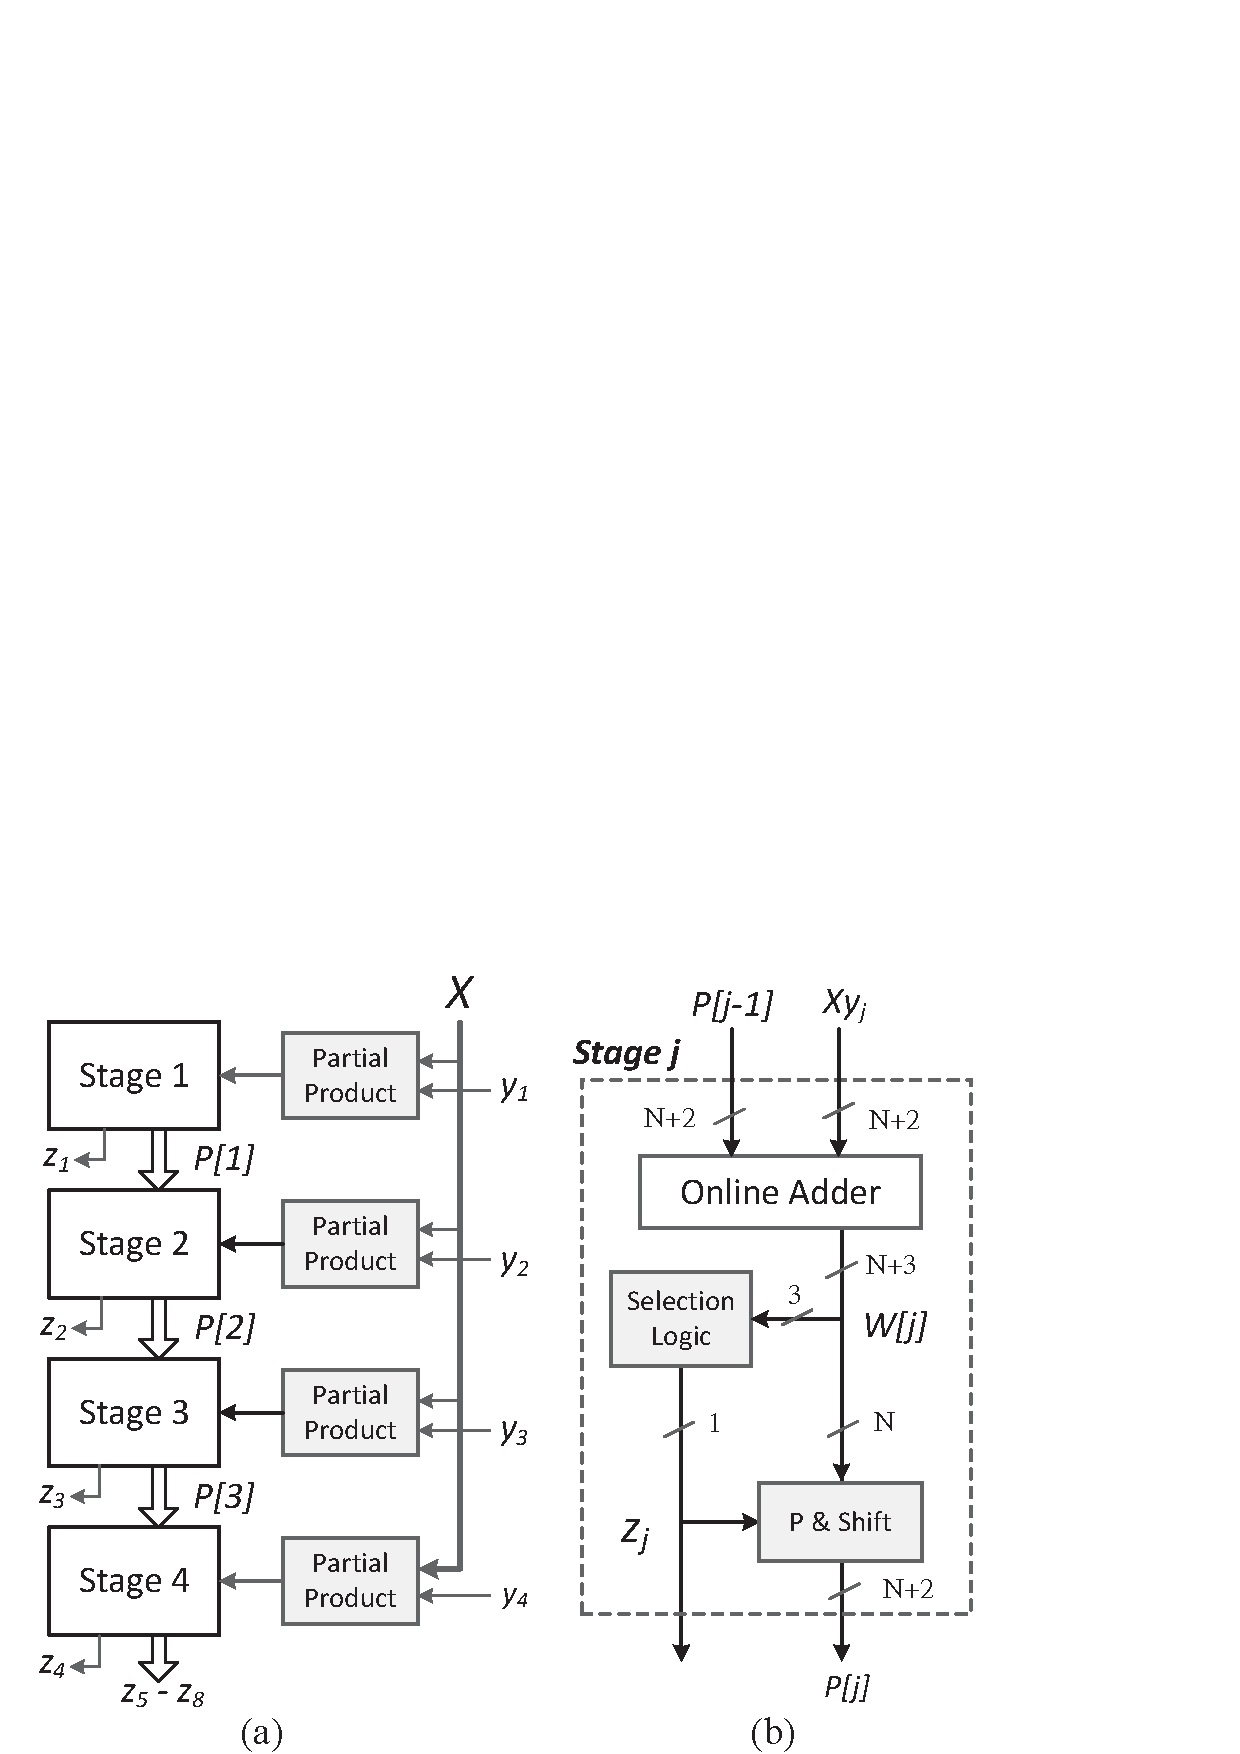
\includegraphics[width=.5\textwidth]{./Figures/ParallelMult_Structure.pdf}
	\caption{(a) Structural diagram of a 4-digit online multiplier using the proposed algorithm. (b) Structure of one stage. The word-length of all signals are labelled in terms of the number of digits. $N$ denotes the word-length of the input signal.}
	\label{Fig:PMStructure}
\end{figure}

\subsection{Structure Optimization for the MSD Half of the Results}

Normally the OM is connected with other arithmetic operators in real applications. If the outputs of an OM is utilized for subsequent operations, only the most significant half of the products are required to maintain the consistency of word-length between inputs and outputs. In the conventional multiplier with standard binary arithmetic, this is achieved by either truncating or rounding the least significant half of the products. However both the computation time and the structure remains unchanged, because the results are generated from LSDs. 

In comparison, the online multiplier offers the possibility to optimize the structure to a further extent if only the MSD half of the results are required, as the results are generated initially from the MSD. The modified structure diagram is illustrated in Fig.~\ref{Fig:PMStructure_MSDhalf}(a). The word-length of the online adder in a given Stage $j$ can be reduced, as shown in Fig.~\ref{Fig:PMStructure_MSDhalf}(b). This is because there is no carry propagation in the online adder, and all digits of the online adder are obtained in parallel.

\begin{figure}[tbp]
	\centering
	\includegraphics[width=.5\textwidth]{./Figures/ParallelMult_MSDhalf.pdf}
	\caption{(a) Modified structure of a 4-digit online multiplier which only generates the most significant 4-digit result. }
	\label{Fig:PMStructure_MSDhalf}
\end{figure}

\subsection{Performance Analysis}


\section{Results}



% Note that IEEE typically puts floats only at the top, even when this
% results in a large percentage of a column being occupied by floats.


% An example of a double column floating figure using two subfigures.
% (The subfig.sty package must be loaded for this to work.)
% The subfigure \label commands are set within each subfloat command, the
% \label for the overall figure must come after \caption.
% \hfil must be used as a separator to get equal spacing.
% The subfigure.sty package works much the same way, except \subfigure is
% used instead of \subfloat.
%
%\begin{figure*}[!t]
%\centerline{\subfloat[Case I]\includegraphics[width=2.5in]{subfigcase1}%
%\label{fig_first_case}}
%\hfil
%\subfloat[Case II]{\includegraphics[width=2.5in]{subfigcase2}%
%\label{fig_second_case}}}
%\caption{Simulation results}
%\label{fig_sim}
%\end{figure*}
%
% Note that often IEEE papers with subfigures do not employ subfigure
% captions (using the optional argument to \subfloat), but instead will
% reference/describe all of them (a), (b), etc., within the main caption.


% An example of a floating table. Note that, for IEEE style tables, the 
% \caption command should come BEFORE the table. Table text will default to
% \footnotesize as IEEE normally uses this smaller font for tables.
% The \label must come after \caption as always.
%
%\begin{table}[!t]
%% increase table row spacing, adjust to taste
%\renewcommand{\arraystretch}{1.3}
% if using array.sty, it might be a good idea to tweak the value of
% \extrarowheight as needed to properly center the text within the cells
%\caption{An Example of a Table}
%\label{table_example}
%\centering
%% Some packages, such as MDW tools, offer better commands for making tables
%% than the plain LaTeX2e tabular which is used here.
%\begin{tabular}{|c||c|}
%\hline
%One & Two\\
%\hline
%Three & Four\\
%\hline
%\end{tabular}
%\end{table}


% Note that IEEE does not put floats in the very first column - or typically
% anywhere on the first page for that matter. Also, in-text middle ("here")
% positioning is not used. Most IEEE journals/conferences use top floats
% exclusively. Note that, LaTeX2e, unlike IEEE journals/conferences, places
% footnotes above bottom floats. This can be corrected via the \fnbelowfloat
% command of the stfloats package.



\section{Conclusion}
The conclusion goes here.




% conference papers do not normally have an appendix


% use section* for acknowledgement
\section*{Acknowledgment}




% trigger a \newpage just before the given reference
% number - used to balance the columns on the last page
% adjust value as needed - may need to be readjusted if
% the document is modified later
%\IEEEtriggeratref{8}
% The "triggered" command can be changed if desired:
%\IEEEtriggercmd{\enlargethispage{-5in}}

% references section

\bibliographystyle{./IEEEtran}
\bibliography{./IEEEabrv,./Reference.bib}

\end{document}


